This configuration manual is also published online in the LandPortal's Drupal repository at GitHub\footnote{\url{https://github.com/weso/landportal-drupal}}.

Here are the instructions for configuring the new \textit{LandPortal}.  All of the following steps can be easily followed using the Drupal's administration interface.  To use the administration interface you must log into the \textit{LandPortal} using an account with administrator privileges.

\textbf{Important notice}:  sometimes in this manual, there will appear some paths.  Those paths are used to easily navigate for the Drupal's administration interface.  Each path is relative to the current server host.  This means that, if the current server host is \textit{landportal.weso.es}, the path \textit{admin/appearance} really means: \textit{landportal.weso.es/admin/appearance}.


\subsection{Enable the \textit{LandPortal} theme}
The new \textit{LandPortal} appearance is provided by a custom theme created specially for the occasion.  The theme receives the name of ``\textit{book}''.  To enable the ``\textit{book}'' theme go to the tab \textit{Appearance} in the top bar of the administration interface.

Once in the \textit{Appearance} tab, scroll down to the bottom of the page, and in the section \textit{disabled themes} click ``\textit{Enable and set default}'' in the \textit{Book theme for LandPortal}.  Now, the ``\textit{book}'' theme is used by default in all pages\footnote{For security reasons the administration interface will still use the default Drupal theme.}


\subsubsection{Configuring the \textit{favicon}}
The \textit{favicon} is a little icon that shows in the browser's tabs and in the browser's bookmark section, representing the entire site.  The new \textit{LandPortal} has a nice \textit{favicon} wich can be easily enabled:
\begin{enumerate}
	\item Go to the path \textit{admin/appearance/settings}
	\item Go to the section \textit{Shortcut icon settings} and uncheck the option \textit{Use the default shortcut icon}
	\item In the field \textit{Path to custom icon} write \textbf{sites/all/themes/book/favicon.png}
\end{enumerate}

The image \ref{fig:manual_configuracion_favicon} shows how those options should look like.
\begin{figure}[h]
	\centering
	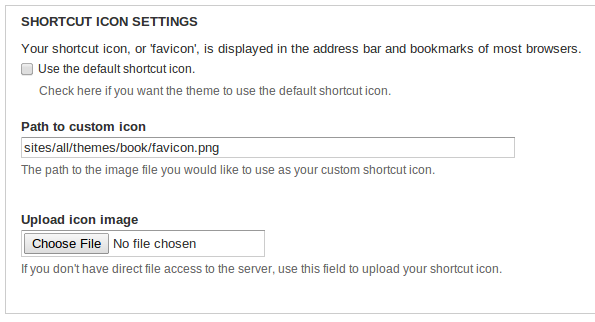
\includegraphics[width=\textwidth]{manual_configuracion/favicon}
	\caption{\textit{LandPortal}'s favicon configuration}
	\label{fig:manual_configuracion_favicon}
\end{figure}

\subsubsection{Configuring \textit{home} and \textit{error} pages}
The new \textit{LandPortal} has a nice home and error pages.  The home page is called \textit{hub}, aid it has been designed to be the entry point to the new \textit{LandPortal}.  The error page shows a nice compass to entertain the users when an error happens.  To enable those views take the following steps:
\begin{enumerate}
	\item Go to the path \textit{admin/config/system/site-information}
	\item In the field \textit{Default front page} write \textbf{home}
	\item In the \textit{ERROR PAGES} fields write \textbf{e404}
\end{enumerate}

The image \ref{fig:manual_configuracion_homeanderror} shows how those fields should look like.
\begin{figure}[h]
	\centering
	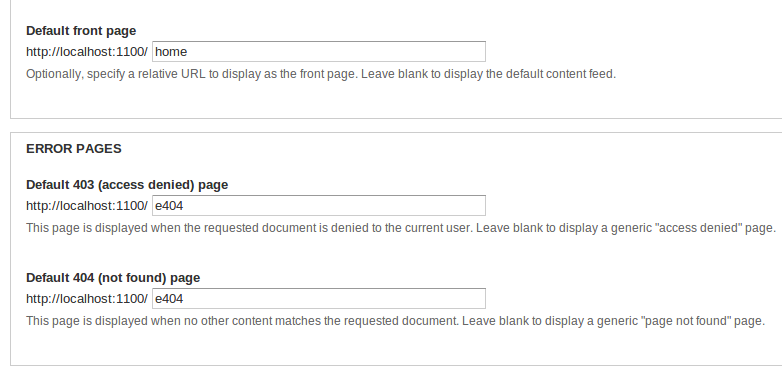
\includegraphics[width=\textwidth]{manual_configuracion/home_and_error_pages}
	\caption{\textit{LandPortal}'s home and error pages}
	\label{fig:manual_configuracion_homeanderror}
\end{figure}

\subsubsection{Configuring the \textit{login} redirection}
The default behaviour of Drupal consists of redirecting a user to it's profile page after he has logged into the system.  As stated in the previous section, the \textit{hub} page has been designed as the entry point for the new \textit{LandPortal}.  We want to override the Drupal's default behaviour to load our \textit{hub} page after a user logs into the system.\\
Two steps are required to achieve this:
\begin{enumerate}
	\item Go to the path \textit{admin/config/system/actions}.  In the bottom page you will see the page creation form.  Chose the option \textit{redirect to URL} in the dropdown menu and click the button \textit{Create}.  A new page will load in which you can set the action label (we suggest something readable, for example: ``\textit{LandPortal redirect on login}'').  In the field \textit{url} write \textbf{home} (the \textit{hub} path).  The image \ref{fig:manual_configuracion_userredirection} shows how those options should look.
	\item Go to the path \textit{admin/structure/trigger/user} and in the option \textit{After an user has logged in} select the action created in the previous step.  Then click the button \textit{assign}.
\end{enumerate}

\begin{figure}[h]
	\centering
	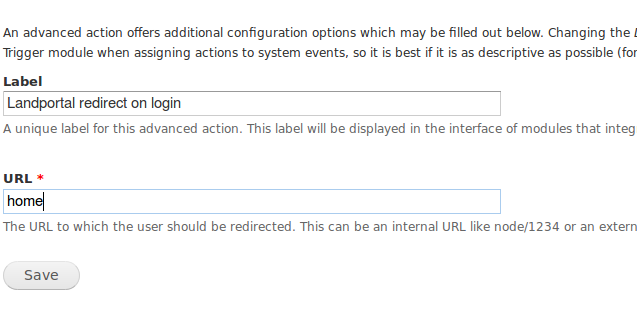
\includegraphics[width=\textwidth]{manual_configuracion/user_redirection}
	\caption{User redirection configuration}
	\label{fig:manual_configuracion_userredirection}
\end{figure}



\subsection{Import the \textit{taxonomy terms}}
The \textit{LandDebate} uses 5 different \textit{taxonomies} or \textit{vocabulary} to classify the different contents.
\begin{itemize}
	\item Continents
	\item Countries
	\item Regions
	\item Debate status
	\item Topics
\end{itemize}
Each of those \textit{taxonomies} is populated by \textit{terms}.  Unfortunately, those \textit{terms} must be imported in a manual way (the import process only needs to be done once).  The following steps explain how to import the \textit{taxonomy terms}:
\begin{enumerate}
	\item Go to the path \textit{admin/structure/taxonomy}
	\item Click the button \textit{CSV IMPORT} in the right upper side
	\item Choose \textit{Translation} as the type of import.  In the field \textit{list of languages} write \textbf{und, es, fr}
	\item Paste the taxonomy terms\footnote{\url{https://github.com/weso/landportal-drupal/blob/develop/taxonomy_terms/continents.csv}} into the text box called \textit{Terms to import}
	\item in the field \textit{vocabulary choice} select the taxonomy \textbf{Continents}
	\item Repeat the above steps with the \textbf{countries}\footnote{\url{https://github.com/weso/landportal-drupal/blob/develop/taxonomy_terms/countries.csv}}, \textbf{topics}\footnote{\url{https://github.com/weso/landportal-drupal/blob/develop/taxonomy_terms/topics.csv}}, \textbf{regions}\footnote{\url{https://github.com/weso/landportal-drupal/blob/develop/taxonomy_terms/regions.csv}} and \textbf{debate status}\footnote{\url{https://github.com/weso/landportal-drupal/blob/develop/taxonomy_terms/debate_status.csv}} taxonomies.  Don't forget to select the corresponding destiny taxonomy in each case.
\end{enumerate}

The images \ref{fig:manual_configuracion_taxonomyimport2} and \ref{fig:manual_configuracion_taxonomyimport} illustrate some of the above steps.

\begin{figure}[h]
	\centering
	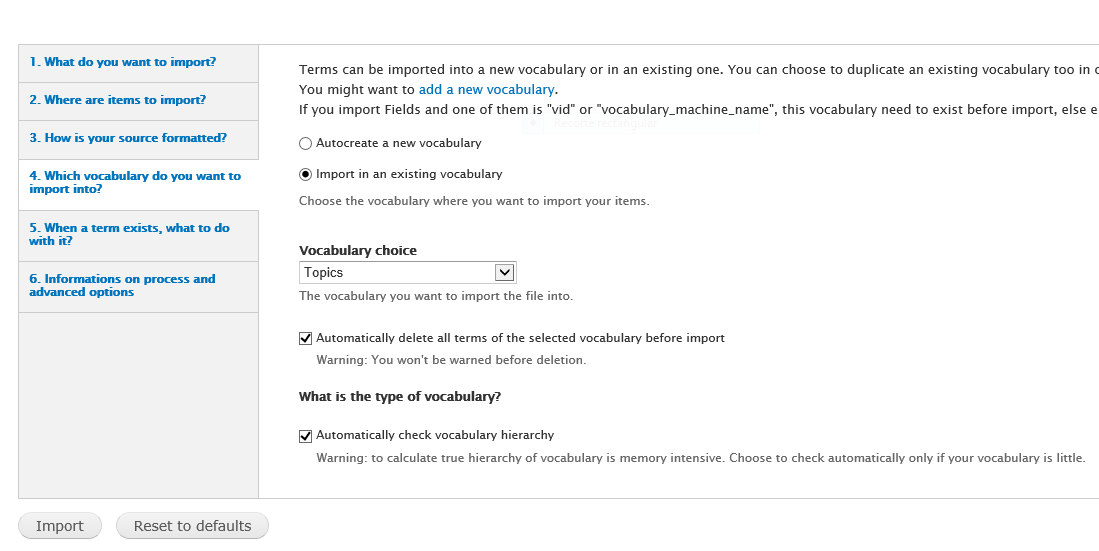
\includegraphics[width=\textwidth]{manual_configuracion/taxonomy_import}
	\caption{Taxonomy import destiny vocabulary selection}
	\label{fig:manual_configuracion_taxonomyimport}
\end{figure}
\begin{figure}[h]
	\centering
	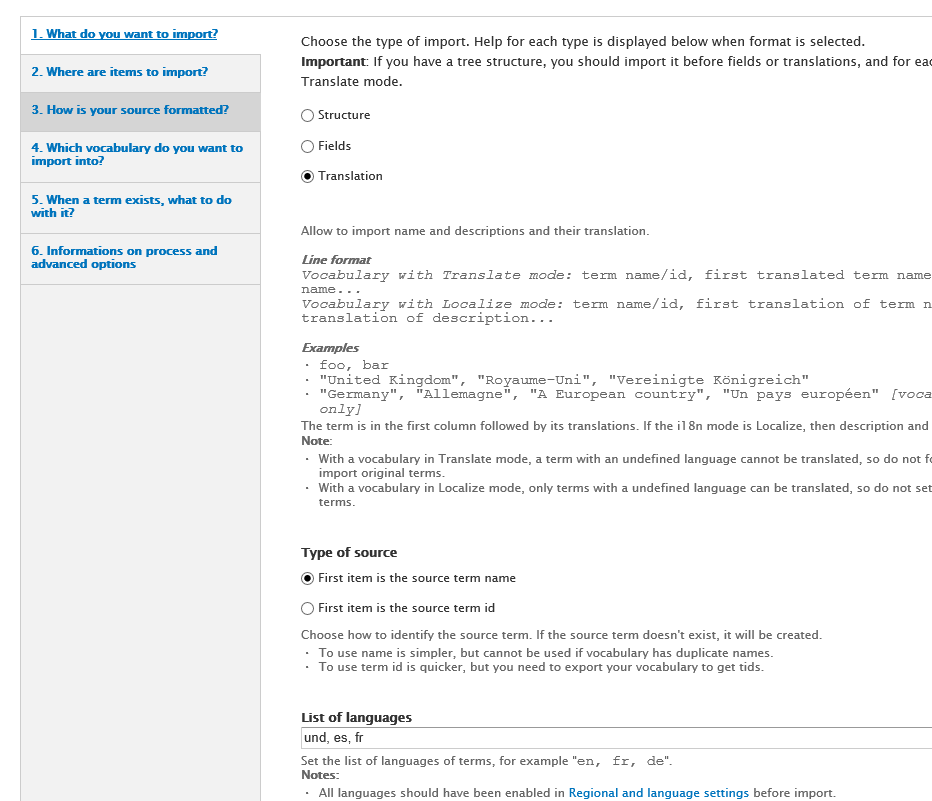
\includegraphics[width=\textwidth]{manual_configuracion/taxonomy_import2}
	\caption{Taxonomy import type and languages configuration}
	\label{fig:manual_configuracion_taxonomyimport2}
\end{figure}



\subsection{Configure the content types}
A new Drupal installation creates two content types by default, those content types are called \textit{Article} and \textit{Basic page} and will not be used into the new \textit{LandPortal}, so they can be omitted or deleted without problem.  The content types can be accessed in the path \textit{admin/structure/types}.

\subsubsection{Configure the \textit{Blog posts}}
The \textit{Blog posts} content type can be configured in the path \textit{admin/structure/types/manage/blog-post}
\begin{itemize}
	\item Change the option \textit{preview before submitting} to \textit{disabled}
	\item In the section \textit{comment settings} uncheck the options \textit{Threading} and \textit{Allow comment title}
	\item In the section \textit{comment settings} set the option \textit{Preview comment} to \textbf{Disabled}
\end{itemize}

\subsubsection{Configure the \textit{Debates}}
The \textit{Debates} content type can be configured in the path \textit{admin/structure/types/manage/debate}
\begin{itemize}
	\item Change the option \textit{preview before submitting} to \textit{disabled}
	\item In the section \textit{comment settings} set the option \textit{Default comment status for new content} to \textbf{Closed}
	\item In the section \textit{comment settings} set the option \textit{Preview comment} to \textbf{Disabled}
\end{itemize}

\subsubsection{Configure the \textit{Events}}
The \textit{Events} content type can be configured in the path \textit{admin/structure/types/manage/event}
\begin{itemize}
	\item Change the option \textit{preview before submitting} to \textit{disabled}
	\item In the section \textit{comment settings} uncheck the options \textit{Threading} and \textit{Allow comment title}
	\item In the section \textit{comment settings} set the option \textit{Preview comment} to \textbf{Disabled}
	\item In the section \textit{comment settings} set the option \textit{Default comment status for new content} to \textbf{Hidden}
\end{itemize}

\subsubsection{Configure the \textit{News}}
The \textit{News} content type can be configured in the path \textit{admin/structure/types/manage/news}.  The configuration for this content type is the same as the configuration for the \textit{Events}.

\subsubsection{Configure the \textit{Organizations}}
The \textit{Organizations} content type can be configured in the path \textit{admin/structure/types/manage/organization}.  The configuration for this content type is the same as the configuration for the \textit{Events}.



\subsection{Configure the search}
\subsubsection{Connect to the \textit{Apache Solr} service}
The new \textit{LandPortal} uses \textit{Apache Solr} to provide a high quality search service.  The following steps are required to configure \textit{Apache Solr}:
\begin{itemize}
	\item Go to the \textit{Configuration} tab in the top bar of the administration interface
	\item Go to the option \textit{Apache Solr search} in the administration panel
	\item Go to the tab \textit{Settings} and click the link named \textit{edit}
	\item In the field \textit{Solr server URL} write \textbf{http://localhost:8983/solr/drupal} and click the button \textit{Save}
\end{itemize}
The image \ref{fig:manual_configuracion_solrconnection} shows how the \textit{Apache Solr} search server should look after its configuration.  The green colour means that Drupal has successfully contacted Solr.
\begin{figure}[h]
	\centering
	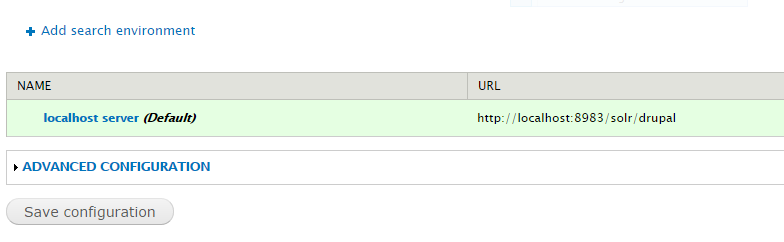
\includegraphics[width=\textwidth]{manual_configuracion/solr_connection}
	\caption{Solr connection configuration result}
	\label{fig:manual_configuracion_solrconnection}
\end{figure}

\subsubsection{Set \textit{Apache Solr} as the default search provider}
Drupal supports multiple search providers.  To use \textit{Apache Solr} as the default search provide in the new \textit{LandPortal} take the following steps:
\begin{enumerate}
	\item Go to the path \textit{admin/config/search/settings}
	\item In the section \textit{Default search module} choose the option \textit{Apache Solr search}
\end{enumerate}
The image \ref{fig:manual_configuracion_solr} shows how those options should look like.
\begin{figure}[h]
	\centering
	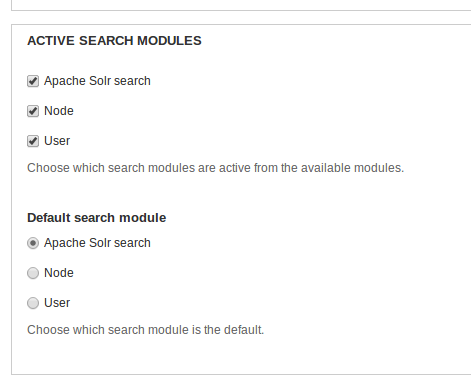
\includegraphics[width=\textwidth]{manual_configuracion/solr_as_default}
	\caption{Solr as the default search server configuration}
	\label{fig:manual_configuracion_solr}
\end{figure}


\subsection{Configure the \textit{WYSIWYG} editor}
The \textit{WYSIWYG} module allows Drupal to show a nice text editor component in which the users can easily format the text and insert images.  To enable this module take the following steps:
\begin{enumerate}
	\item Go to the path \textit{admin/config/content/wysiwyg}
	\item For each profile choose the editor \textit{markItUp 1.1.14}
	\item After selecting the editor you can change its options and choose which buttons to show.  We suggest enabling all the buttons for the best user experience.
\end{enumerate}

The image \ref{fig:manual_configuracion_wysiwyg} shows how to enable those buttons.
\begin{figure}[h]
	\centering
	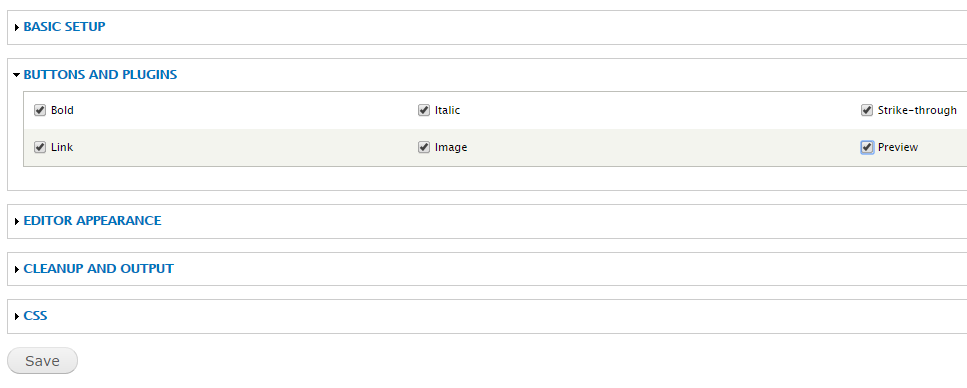
\includegraphics[width=\textwidth]{manual_configuracion/wysiwyg}
	\caption{WYSIWYG text editor configuration}
	\label{fig:manual_configuracion_wysiwyg}
\end{figure}